\documentclass[tikz,border=8pt]{standalone}
\usetikzlibrary{arrows.meta,positioning,fit,decorations.pathreplacing}
\begin{document}
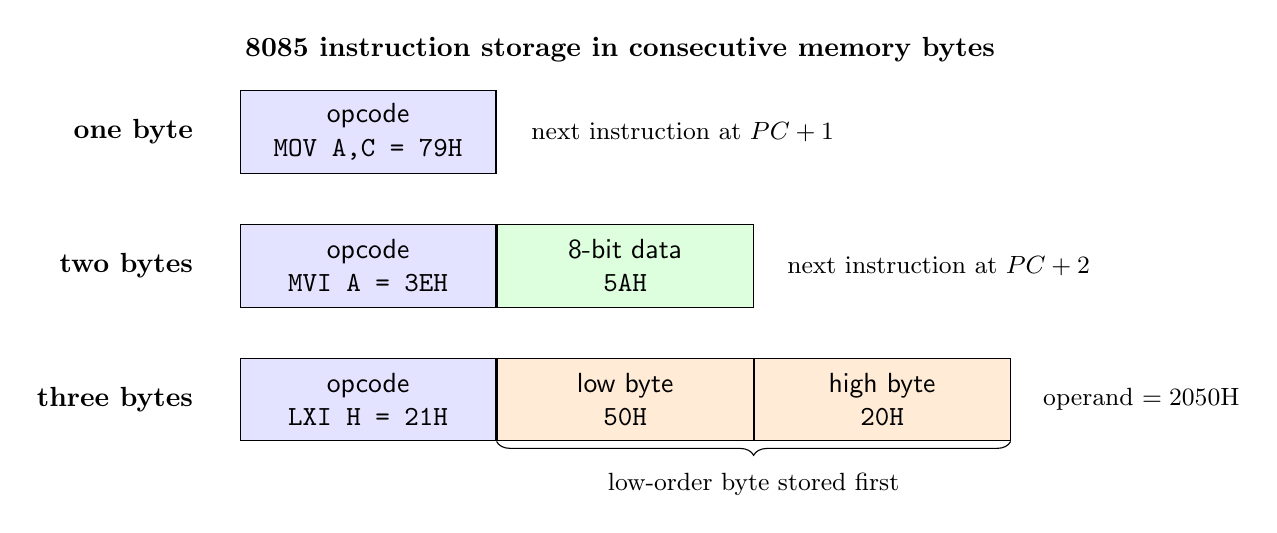
\begin{tikzpicture}[
  font=\sffamily,
  >=Latex,
  byte/.style={draw,minimum width=3.25cm,minimum height=1.05cm,align=center},
  label/.style={font=\bfseries,anchor=east},
  note/.style={font=\small,anchor=west}
]
\node[label] at (0,2.5) {one byte};
\node[byte,fill=blue!11] (o1) at (2.1,2.5) {opcode\\\texttt{MOV A,C = 79H}};
\node[note] at (4.05,2.5) {next instruction at $PC+1$};

\node[label] at (0,0.8) {two bytes};
\node[byte,fill=blue!11] (o2) at (2.1,0.8) {opcode\\\texttt{MVI A = 3EH}};
\node[byte,fill=green!13,right=0pt of o2] (d2) {8-bit data\\\texttt{5AH}};
\node[note] at (7.30,0.8) {next instruction at $PC+2$};

\node[label] at (0,-0.9) {three bytes};
\node[byte,fill=blue!11] (o3) at (2.1,-0.9) {opcode\\\texttt{LXI H = 21H}};
\node[byte,fill=orange!16,right=0pt of o3] (lo) {low byte\\\texttt{50H}};
\node[byte,fill=orange!16,right=0pt of lo] (hi) {high byte\\\texttt{20H}};
\node[note] at (10.55,-0.9) {operand $=2050\mathrm{H}$};

\draw[decorate,decoration={brace,mirror,amplitude=5pt}]
  (lo.south west) -- (hi.south east)
  node[midway,below=8pt,font=\small] {low-order byte stored first};
\node[font=\bfseries] at (5.3,3.55) {8085 instruction storage in consecutive memory bytes};
\end{tikzpicture}
\end{document}
